\documentclass{beamer}
\usepackage{graphicx}
\usepackage{xcolor}
\usepackage{tikz}
\usepackage{amsmath}
\usepackage{pgfplots}
\pgfplotsset{compat=1.18}

\definecolor{purpleblue}{RGB}{80, 80, 180}
\definecolor{novelPurple}{RGB}{98, 54, 255}
\definecolor{softPurple}{RGB}{180, 170, 255}
\definecolor{softGray}{RGB}{235, 235, 245}
\definecolor{lightText}{RGB}{90, 90, 110}

\usetheme{Madrid}
\usecolortheme{dolphin}
\graphicspath{{static/course_materials/}{static/hard/}{./}}

\setbeamerfont{title}{size=\Large,series=\bfseries}
\setbeamerfont{frametitle}{size=\LARGE,series=\bfseries}
\setbeamercolor{frametitle}{fg=white, bg=novelPurple}
\setbeamercolor{title}{fg=white, bg=purpleblue}

\title[Test II]{\textbf{Test II}}
\author{\textbf{Jack Zeng}}
\institute{\textcolor{white}{\textbf{Novel Prep}}}
\date{\today}

\begin{document}

\begin{frame}
    \titlepage
    \vfill
    \begin{flushright}
        \textcolor{purpleblue}{\Huge \textbf{Novel Prep}}
    \end{flushright}
\end{frame}

\begin{frame}
    \begin{tikzpicture}[remember picture, overlay]
        \shade[top color=softPurple, bottom color=softGray]
            (current page.north west) rectangle (current page.south east);
        \node[align=center] at (current page.center) {
            {\Huge\bfseries\textcolor{purpleblue}{Novel Prep}} \\[0.5cm]
            {\Large\itshape\textcolor{lightText}{Phase 3 · Test II}}
        };
    \end{tikzpicture}
\end{frame}

\begin{frame}{Overview}
    \tableofcontents
\end{frame}

\begin{frame}
\section{Test II}
    \begin{tikzpicture}[remember picture, overlay]
        \shade[top color=softPurple, bottom color=softGray]
            (current page.north west) rectangle (current page.south east);
        \node[align=center] at (current page.center) {
            {\LARGE\bfseries\textcolor{purpleblue}{Test II}} \\[0.5cm]
            {\Large\itshape\textcolor{lightText}{24 word-problem training challenges}}
        };
    \end{tikzpicture}
\end{frame}

% --- Question 1 ---
\begin{frame}{Question 1}
\small
For the equation, \(b\) and \(c\) are constants. For any real number \(t\), the point \(\left(\dfrac{-2t + 4}{3}, t\right)\) lies on the graph of the equation \(bx + 3y = c\).
What is the value of \(c\)?
\vspace{0.35cm}
\begin{enumerate}
    \item[A.] \(-2\)
    \item[B.] \(4\)
    \item[C.] \(6\)
    \item[D.] \(12\)
\end{enumerate}
\end{frame}
\begin{frame}{Answer 1}
\small
\textbf{Correct Answer:} C
\end{frame}

% --- Question 2 ---
\begin{frame}{Question 2}
\small
The function \(q\) is defined by
\[
q(x) = a|x - 9|^2 - 87|x - 9| + b,
\]
where \(a\) and \(b\) are constants and \(a > b > 87\). In the \(xy\)-plane, the graph of \(y = q(x)\) contains the points \((639, h)\) and \((-621, k)\), where \(h\) and \(k\) are constants.
What is the value of \(9(-639)^{h-k} + 621(9)^{k-h}\)?
\end{frame}
\begin{frame}{Answer 2}
\small
\textbf{Final Answer:} $\boxed{630}$
\end{frame}

% --- Question 3 ---
\begin{frame}{Question 3}
\small
In the given equation, \(a\) and \(b\) are positive constants. A solution to the equation is \(x = 42\).
\[
x(9x - 2a) + b(9x - 2a) - (x + b) = 0
\]
What is the value of \(a\)?
\end{frame}
\begin{frame}{Answer 3}
\small
\textbf{Final Answer:} $\boxed{188.5}$
\end{frame}

% --- Question 4 ---
\begin{frame}{Question 4}
\small
The function \(z\) is defined by
\[
z(w) = (0.829)^{2w}.
\]
The value of \(z(w)\) decreases by \(p\%\) for each increase by \(1\) in the value of \(w\). Which of the following is closest to the value of \(p\)?
\vspace{0.35cm}
\begin{enumerate}
    \item[A.] \(0.171\)
    \item[B.] \(0.829\)
    \item[C.] \(17.1\)
    \item[D.] \(31.3\)
\end{enumerate}
\end{frame}
\begin{frame}{Answer 4}
\small
\textbf{Correct Answer:} D
\end{frame}

% --- Question 5 ---
\begin{frame}{Question 5}
\small
\begin{center}
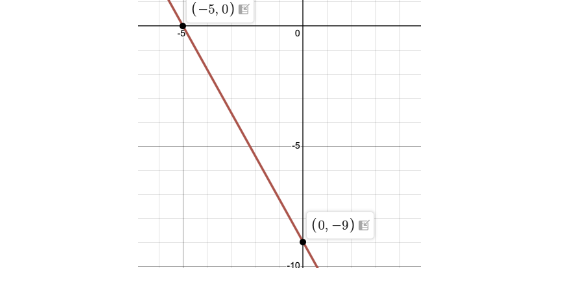
\includegraphics[width=0.72\linewidth]{hard_20_f05_line.png}
\end{center}

The graph of line \(h\) is shown in the \(xy\)-plane. Line \(k\) (not shown) is defined by the equation \(sx + 40y = t\), where \(s\) and \(t\) are constants. If line \(k\) is graphed in this \(xy\)-plane, the result is a graph of two linear equations. This system of two linear equations has no solution. Which of the following is NOT a possible value of \(t\)?
\vspace{0.35cm}
\begin{enumerate}
    \item[A.] \(-360\)
    \item[B.] \(-9\)
    \item[C.] \(72\)
    \item[D.] \(200\)
\end{enumerate}
\end{frame}
\begin{frame}{Answer 5}
\small
\textbf{Correct Answer:} A
\end{frame}

% --- Question 6 ---
\begin{frame}{Question 6}
\small
The function \(h\) is defined by
\[
h(x) = -\sqrt{x^{2} + bx + c},
\]
where \(b\) and \(c\) are constants. The graph of \(y = h(x)\) contains the points \((2, 0)\) and \(\bigl(0, -\sqrt{358}\bigr)\). If \(h(m) = 0\), what is the greatest possible value of \(m\)?
\vspace{0.35cm}
\begin{enumerate}
    \item[A.] \(2\)
    \item[B.] \(177\)
    \item[C.] \(179\)
    \item[D.] \(358\)
\end{enumerate}
\end{frame}
\begin{frame}{Answer 6}
\small
\textbf{Correct Answer:} C
\end{frame}

% --- Question 7 ---
\begin{frame}{Question 7}
\small
The functions \(f\) and \(g\) are defined by the equations shown, where \(a\) and \(b\) are integer constants, \(a < b\), and \(b < 0\). If \(y = f(x)\) and \(y = g(x)\) are graphed in the \(xy\)-plane, which of the following equations displays, as a constant or coefficient, the \(y\)-coordinate of the \(y\)-intercept of the graph of the corresponding function?
\begin{itemize}
\item[I.] \(f(x) = a(2.1)^{x + b}\)
\item[II.] \(g(x) = a(2.1)^{x} + b\)
\end{itemize}
\vspace{0.35cm}
\begin{enumerate}
    \item[A.] I only
    \item[B.] II only
    \item[C.] I and II
    \item[D.] Neither I nor II
\end{enumerate}
\end{frame}
\begin{frame}{Answer 7}
\small
\textbf{Correct Answer:} D
\end{frame}

% --- Question 8 ---
\begin{frame}{Question 8}
\small
The function \(f\) is defined by
\[
f(x) = \dfrac{x^{2} + ax + b}{2x + c},
\]
where \(a\), \(b\), and \(c\) are constants. The graph of \(y = f(x)\) does not intersect the line \(x = 4\). If \(f(5) = f(6) = 0\), what is the value of \(a + b + c\)?
\vspace{0.35cm}
\begin{enumerate}
    \item[A.] \(10\)
    \item[B.] \(11\)
    \item[C.] \(12\)
    \item[D.] \(13\)
\end{enumerate}
\end{frame}
\begin{frame}{Answer 8}
\small
\textbf{Correct Answer:} B
\end{frame}

% --- Question 9 ---
\begin{frame}{Question 9}
\small
The positive number \(a\) is \(2{,}106\%\) of the sum of the positive numbers \(b\) and \(c\), and \(b\) is \(81\%\) of \(c\).
What percent of \(b\) is \(a\)?
\vspace{0.35cm}
\begin{enumerate}
    \item[A.] \(4{,}706\%\)
    \item[B.] \(47.06\%\)
    \item[C.] \(470{,}600\%\)
    \item[D.] \(47{,}060\%\)
\end{enumerate}
\end{frame}
\begin{frame}{Answer 9}
\small
\textbf{Correct Answer:} A
\end{frame}

% --- Question 10 ---
\begin{frame}{Question 10}
\small
Point \(N\) lies on a unit circle in the \(xy\)-plane and has coordinates \((1, 0)\). Point \(O\) is the center of the circle and has coordinates \((0, 0)\). Point \(M\) also lies on the unit circle, and the measure of angle \(\angle NOM\) is \(\dfrac{266\pi}{3}\) radians. If the coordinates of point \(M\) are \((a, b)\), where \(a\) and \(b\) are constants, what is the value of \(a\)?
\vspace{0.35cm}
\begin{enumerate}
    \item[A.] \(\dfrac{1}{2}\)
    \item[B.] \(\dfrac{\sqrt{3}}{2}\)
    \item[C.] \(-\dfrac{1}{2}\)
    \item[D.] \(-\dfrac{\sqrt{3}}{2}\)
\end{enumerate}
\end{frame}
\begin{frame}{Answer 10}
\small
\textbf{Correct Answer:} C
\end{frame}

% --- Question 11 ---
\begin{frame}{Question 11}
\small
In the given equation, \(a\) and \(b\) are positive constants. The sum of the solutions to the given equation is \(k(6a + b)\), where \(k\) is a constant. What is the value of \(k\)?
\[
24x^{2} - (12a + 2b)x + ab = 0
\]
\vspace{0.35cm}
\begin{enumerate}
    \item[A.] \(\dfrac{1}{12}\)
    \item[B.] \(-\dfrac{1}{12}\)
    \item[C.] \(12\)
    \item[D.] \(-12\)
\end{enumerate}
\end{frame}
\begin{frame}{Answer 11}
\small
\textbf{Correct Answer:} A
\end{frame}

% --- Question 12 ---
\begin{frame}{Question 12}
\small
In triangle \(ABC\), the measure of angle \(B\) is \(90^\circ\) and \(BD\) is an altitude of the triangle. The length of \(AB = 15\), and the length of \(AC\) is \(23\) greater than the length of \(AB\). What is the value of \(\dfrac{BC}{BD}\)?
\vspace{0.35cm}
\begin{enumerate}
    \item[A.] \(\dfrac{15}{38}\)
    \item[B.] \(\dfrac{15}{23}\)
    \item[C.] \(\dfrac{23}{15}\)
    \item[D.] \(\dfrac{38}{15}\)
\end{enumerate}
\end{frame}
\begin{frame}{Answer 12}
\small
\textbf{Correct Answer:} D
\end{frame}

% --- Question 13 ---
\begin{frame}{Question 13}
\small
A right square pyramid has a height of \(11\) centimeters (cm). A second right square pyramid has a height of \(22\) centimeters. The area of the bases of each of the two pyramids is \(100\,\text{cm}^{2}\).
Which of the following is closest to the difference in the surface area of the second pyramid and the surface area of the first pyramid, in \(\text{cm}^{2}\)?
\vspace{0.35cm}
\begin{enumerate}
    \item[A.] \(209\)
    \item[B.] \(220\)
    \item[C.] \(367\)
    \item[D.] \(551\)
\end{enumerate}
\end{frame}
\begin{frame}{Answer 13}
\small
\textbf{Correct Answer:} A
\end{frame}

% --- Question 14 ---
\begin{frame}{Question 14}
\small
A researcher investigated two species of mites: a predator and its prey. At the start of a week, there was an equal number of the two species. At the end of the week:
\begin{itemize}
\item The number of prey had increased by \(2{,}700\%\) of the number of prey at the start of the week.
\item The number of predators had increased by \(180\%\) of the number of predators at the start of the week.
\end{itemize}
The number of prey at the end of the week was \(p\%\) greater than the number of predators at the end of the week. What is the value of \(p\)?
\vspace{0.35cm}
\begin{enumerate}
    \item[A.] \(9\)
    \item[B.] \(90\)
    \item[C.] \(900\)
    \item[D.] \(9{,}000\)
\end{enumerate}
\end{frame}
\begin{frame}{Answer 14}
\small
\textbf{Correct Answer:} C
\end{frame}

% --- Question 15 ---
\begin{frame}{Question 15}
\small
A beekeeper's initial observation of the population of a certain bee colony was \(1{,}100\) bees. The beekeeper set a goal to increase the population to \(2{,}600\) bees.
The beekeeper uses a model that predicts the population of this bee colony:
\begin{itemize}
\item begins at \(1{,}100\)
\item increases by \(120\) bees per week in the first two weeks
\item then increases by \(180\) bees per week until the goal is reached
\end{itemize}
According to this model, at the end of week \(w\) after the initial observation, where \(w > 2\), which of the following functions gives the predicted number of bees still needed to reach the beekeeper's goal?
\vspace{0.35cm}
\begin{enumerate}
    \item[A.] \(p(w) = 2600 - 180w\)
    \item[B.] \(p(w) = 2480 + 180w\)
    \item[C.] \(p(w) = 1620 - 180w\)
    \item[D.] \(p(w) = -120 + 180w\)
\end{enumerate}
\end{frame}
\begin{frame}{Answer 15}
\small
\textbf{Correct Answer:} C
\end{frame}

% --- Question 16 ---
\begin{frame}{Question 16}
\small
The speed of a vehicle is increasing at a rate of \(7.3\) meters per second squared. What is this rate, in miles per minute squared, rounded to the nearest tenth? (Use \(1\) mile \(= 1{,}609\) meters.)
\vspace{0.35cm}
\begin{enumerate}
    \item[A.] \(0.3\)
    \item[B.] \(16.3\)
    \item[C.] \(195.8\)
    \item[D.] \(220.4\)
\end{enumerate}
\end{frame}
\begin{frame}{Answer 16}
\small
\textbf{Correct Answer:} B
\end{frame}

% --- Question 17 ---
\begin{frame}{Question 17}
\small
Which of the following expressions has a factor of \(x + 2b\), where \(b\) is a positive integer constant?
\vspace{0.35cm}
\begin{enumerate}
    \item[A.] \(3x^{2} + 7x + 14b\)
    \item[B.] \(3x^{2} + 16x + 14b\)
    \item[C.] \(3x^{2} + 18x + 14b\)
    \item[D.] \(3x^{2} + 25x + 14b\)
\end{enumerate}
\end{frame}
\begin{frame}{Answer 17}
\small
\textbf{Correct Answer:} D
\end{frame}

% --- Question 18 ---
\begin{frame}{Question 18}
\small
In the given system of equations, \(t\) is a constant. If the system has no solution, what is the value of \(t\)?
\[
\begin{aligned}
16x - 20y &= 6y + 8 \\
ty &= 8x + \dfrac{1}{5}
\end{aligned}
\]
\end{frame}
\begin{frame}{Answer 18}
\small
\textbf{Final Answer:} $\boxed{13}$
\end{frame}

% --- Question 19 ---
\begin{frame}{Question 19}
\small
In the given equation, \(k\) is a positive constant. The product of the solutions to the equation is \(72\). What is the value of \(k\)?
\[
\dfrac{5}{9}(5x + 9)\bigl(x + \sqrt{5k + 9}\bigr)\bigl(x - \sqrt{5k + 9}\bigr) = 0
\]
\end{frame}
\begin{frame}{Answer 19}
\small
\textbf{Final Answer:} $\boxed{6.2}$
\end{frame}

% --- Question 20 ---
\begin{frame}{Question 20}
\small
In the \(xy\)-plane, a unit circle with center at the origin \(O\) contains point \(A\) with coordinates \((1, 0)\) and point \(B\) with coordinates \(\left(\dfrac{5}{\sqrt{34}}, -\dfrac{3}{\sqrt{34}}\right)\). If the measure of angle \(AOB\) is \(p\) radians, what is the value of \(\dfrac{\cos p}{\sin p}\)?
\end{frame}
\begin{frame}{Answer 20}
\small
\textbf{Final Answer:} $\boxed{\dfrac{-5}{3}}$
\end{frame}

% --- Question 21 ---
\begin{frame}{Question 21}
\small
A pyramid with square base area of \(36\,\text{m}^{2}\) has a total surface area of \(36 + 12\sqrt{493}\,\text{m}^{2}\). Find the height of the pyramid.
\end{frame}
\begin{frame}{Answer 21}
\small
\textbf{Final Answer:} $\boxed{22}$
\end{frame}

% --- Question 22 ---
\begin{frame}{Question 22}
\small
The height of a right circular cylinder is \(36\) inches, and the circumference of its base is \(360\) inches. Which expression represents the total surface area, in square inches, of the cylinder?
\vspace{0.35cm}
\begin{enumerate}
    \item[A.] \((36)(360) + 2\pi\left(\dfrac{180}{\pi}\right)^{2}\)
    \item[B.] \((36)(360) + \pi\left(\dfrac{180}{\pi}\right)^{2}\)
    \item[C.] \(\pi\left(\dfrac{180}{\pi}\right)^{2}(36)\)
    \item[D.] \((36)(360)\)
\end{enumerate}
\end{frame}
\begin{frame}{Answer 22}
\small
\textbf{Correct Answer:} A
\end{frame}

% --- Question 23 ---
\begin{frame}{Question 23}
\small
\begin{center}
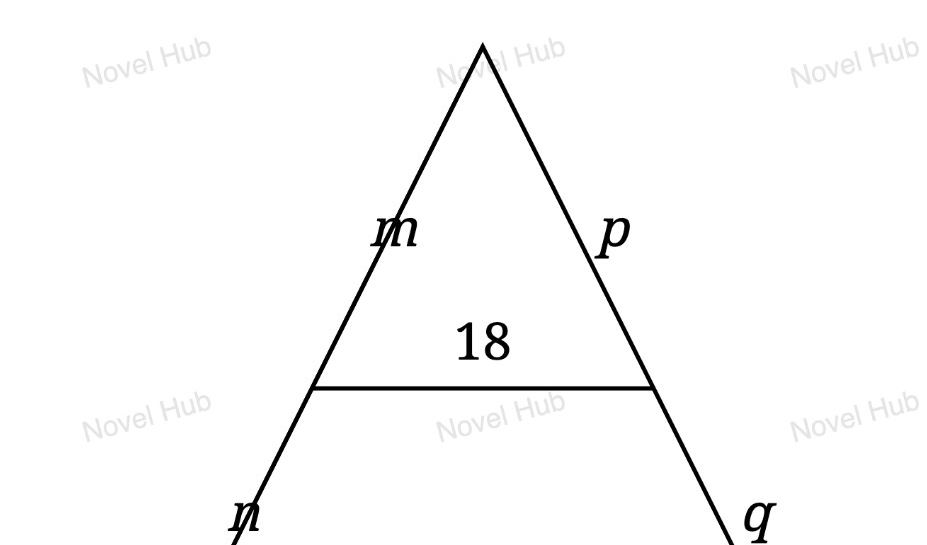
\includegraphics[width=0.62\linewidth]{hard_20_f23_parallel.png}
\end{center}

The parallel line segment divides the other two sides of the triangle into segments of lengths \(m\) and \(n\), and \(p\) and \(q\), respectively. If \(\dfrac{p}{q} = k\) and \(\dfrac{m}{n} = k\), what is the value of \(k\)?
\end{frame}
\begin{frame}{Answer 23}
\small
\textbf{Final Answer:} $\boxed{1.5}$
\end{frame}

% --- Question 24 ---
\begin{frame}{Question 24}
\small
A gear ratio \(r:s\) is the ratio of the number of teeth of two connected gears. The ratio of the number of revolutions per minute (rpm) of two gear wheels is \(s:r\). In the diagram below, Gear A is turned by a motor. The turning of Gear A causes Gears B and C to turn as well.

\begin{center}
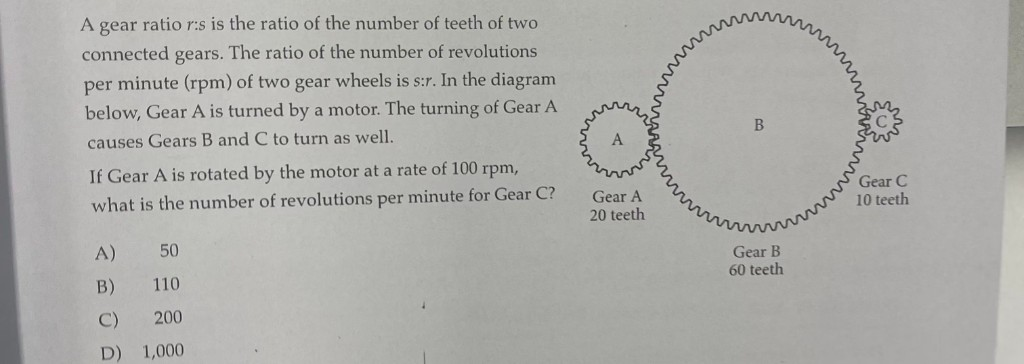
\includegraphics[width=0.88\linewidth]{hard_20_f24_gears.png}
\end{center}

If Gear A is rotated by the motor at a rate of \(100\) rpm, what is the number of revolutions per minute for Gear C?
\vspace{0.35cm}
\begin{enumerate}
    \item[A.] \(50\)
    \item[B.] \(110\)
    \item[C.] \(200\)
    \item[D.] \(1{,}000\)
\end{enumerate}
\end{frame}
\begin{frame}{Answer 24}
\small
\textbf{Correct Answer:} C
\end{frame}

\begin{frame}{}
    \begin{tikzpicture}[remember picture, overlay]
        \shade[top color=novelPurple!40, bottom color=white]
            (current page.north west) rectangle (current page.south east);
        \fill[white, opacity=0.15] (current page.center) circle (5cm);
        \foreach \x in {1,2,3,4,5} {
            \fill[novelPurple, opacity=0.12] (rand*10-5, rand*7-3.5) circle (0.1+\x*0.05);
        }
    \end{tikzpicture}
    \centering
    \vspace{5em}
    {\Huge \textbf{\textcolor{novelPurple}{Thank You!}}} \\[1em]
    {\large \textcolor{gray}{We appreciate your time and focus.}} \\[3em]
    {\LARGE \textbf{\textcolor{novelPurple}{\textsf{Novel Prep}}}}
    \vfill
\end{frame}

\end{document}
